\documentclass[whitelogo]{tudelft-report}

% options avaiable to fix white pages
% http://www.nada.kth.se/~carsten/latex/class.html

% 1) use `openany` to prevent white pages between chapters
% 2)  `oneside`, but this mide have unwanted layout effects as well. like margins are different on uneven pages when printing

% 3) overwrite cleardoublepage, the white pages appear on uneven pages, because the default option with book is openright 
\makeatletter
    \def\cleardoublepage{\clearpage%
        \if@twoside
            \ifodd\c@page\else
                \vspace*{\fill}
                \hfill
                \begin{center}
                % This page intentionally left blank.
                Deze pagina is opzettelijk leeg gelaten.
                \end{center}
                \vspace{\fill}
                \thispagestyle{empty}
                \newpage
                \if@twocolumn\hbox{}\newpage\fi
            \fi
        \fi
    }
\makeatother

\usepackage{changes}
\usepackage{csquotes}
\usepackage[dutch]{babel}
\usepackage{graphicx}
\graphicspath{ {images/} }
% the syle=apa is only in ShareLatex use 'draft' for WIP
\usepackage[backend=biber,sorting=ynt,style=apa]{biblatex}
\DeclareLanguageMapping{dutch}{dutch-apa}
\addbibresource{citations.bib}

\usepackage{pdfpages}

\usepackage{enumitem}
\setlist[enumerate]{itemsep=3pt,parsep=3pt}
\setlist[enumerate,2]{topsep=1pt,parsep=2.5pt}
\setlist[itemize]{itemsep=2pt, parsep=2pt}
\setlength{\parindent}{0pt}
% parskip is done after title page (see pagenr. ~80)

\usepackage{hyperref}
\usepackage{verbatim}
\usepackage{listings}

\usepackage{multirow}

\usepackage{lineno}

\DeclareSourcemap{
    \maps[datatype=bibtex]{
        \map{
            \step[fieldsource=url, notmatch=\regexp{wiki},  final=1]
            \step[fieldset=urldate, null]
        }
    }
}

\usepackage{listings}
\usepackage{listings-golang}

\lstset{ % add your own preferences
    % frame=single,
    basicstyle=\footnotesize,
    % keywordstyle=\color{red},
    % numbers=left,
    % numbersep=5pt,
    showstringspaces=false, 
    stringstyle=\color{blue},
    tabsize=4,
    language=Golang % this is it !
}

\begin{document}
% 
%% Use Roman numerals for the page numbers of the title pages and table of
%% contents.
\frontmatter

%% Uncomment following 19 lines for a cover with a picture on the lower half only
% \title[tudelft-white]{Title}
% \subtitle[tudelft-cyan]{Optional subtitle}
% \author[tudelft-white]{J.\ Random Author}
% \affiliation{Technische Universiteit Delft}
% \coverimage{cover.jpg}
% \titleoffsetx{10cm}
% \titleoffsety{10cm}
% \afiloffsetx{1cm}
% \afiloffsety{18cm}
% \covertext[tudelft-white]{
%    \textbf{Cover Text} \\
%    possibly \\
%    spanning 
%    multiple 
%    lines
%    \vfill
%    ISBN 000-00-0000-000-0
% }
% \makecover

%% Uncomment following 16 lines for a cover with a picture on the lower half only
\title[tudelft-white]{Afstudeeropdracht}
\subtitle[tudelft-black]{Ontwikkel flexibele data-aggregaties voor Shop2market}
\author[tudelft-white]{S.\ Oldeman}
\affiliation{HBO-ICT aan Hogeschool Utrecht}
\coverimage{tank.jpg}
\covertext[tudelft-white]{
    \textbf{Hoe kunnen statistieken}
     voor Adcurve
     actueel blijven en op tijd berekend zijn
    
    % \vfill
    % ISBN 000-00-0000-000-0
}
\setpagecolor{tudelft-cyan}
% \makecover[split]


%% Include an optional title page.
\begin{titlepage}


\begin{center}


%% Print the title in cyan.
{\makeatletter
\largetitlestyle\fontsize{64}{94}\selectfont\@title
\makeatother}

%% Print the optional subtitle in black.
{\makeatletter
\ifx\@subtitle\undefined\else
    \bigskip
   {\tudsffamily\fontsize{22}{32}\selectfont\@subtitle}    
\fi
\makeatother}

\bigskip
\bigskip

door

\bigskip
\bigskip

%% Print the name of the author.
{\makeatletter
%\largetitlefont\Large\bfseries\@author
\largetitlestyle\fontsize{26}{26}\selectfont\@author
\makeatother}

\bigskip
\bigskip

ter verkrijging van de graad van Bachalor HBO-ICT

aan de Hoge school Utrecht,

in het openbaar de verdedigen in Juni, 2016.

\vfill

\begin{tabular}{lll}
    Student nummer: & 1571564 \\
    Project duur: & \multicolumn{2}{l}{18 maart 2016 -- 31 mei 2016} \\
    Afstudeer examinatoren:
        & Dhr.\ M.\ Dumont, & HU, docentbegeleider \\
        & Dhr.\ J.\ W.\ Pauw, & HU \\
        & Dhr.\ M.\ Jorissen, & Shop2market
\end{tabular}
%% Only include the following lines if confidentiality is applicable.


%\centering{
\includegraphics{cover/logo_black}}


\end{center}

\begin{tikzpicture}[remember picture, overlay]
    \node at (current page.south)[anchor=south,inner sep=0pt]{
        
\includegraphics{cover/logo_black}
    };
\end{tikzpicture}

\end{titlepage}



\chapter*{Voorwoord}
\setheader{Voorwoord}

Preface\ldots

\begin{flushright}
{\makeatletter\itshape
    \@author \\
    Utrecht, maart 2016
\makeatother}
\end{flushright}



\setlength{\parskip}{1em}
\chapter{Managementsamenvatting}

In deze thesis is wordt omschreven hoe onderzoek is gedaan naar een nieuwe implementatie voor data aggregatie processen binnen de organisatie Shop2market.

Dit project werd gestart tijdens de ontwikkeling van een nieuwe dienst op basis van bestaande Shop2market platform: Adcurve. Om de gewenste groei van Adcurve te ondersteunen en ruimte bieden voor nieuwe functionaliteiten werd duidelijk dat de huidige oplossing wellicht moest worden onderzocht.


Voor dit project is in de volgende doelstelling omschreven:

\textit{Webwinkel eigenaren moeten in staat zijn om beslissingen te maken op basis van correcte en actuele gegevens in Adcurve. Dit betekent dat de gegevens die Adcurve toont altijd te verklaren zijn en overeenkomen met de werkelijkheid. De data moet op tijd verwerkt zijn, en fouten moeten tijdig hersteld kunnen worden}


In hoofdstuk \ref{ch:project} wordt het project volledig toegelicht, daarnaast is het onderzoeksplan opgesteld. In het onderzoeksplan worden vijf deelvragen behandeld die samen de volgende hoofdvraag beantwoorden, namelijk:

\medskip
{\large \textit{"Hoe verzorgt een nieuwe implementatie voor het up-to-date houden van statistieken in Adcurve zodat gegevens altijd te verklaren zijn?"}}
\medskip

Om de hoofdvraag te beantwoorden zijn de volgende deelvragen geformuleerd

\begin{enumerate}
\item Wat zijn de functionele en niet functionele eisen waaraan de oplossing moet voldoen?
\item Wat zijn toonaangevende methodes en technologieën om statistieken te berekenen, die passen bij de wensen en eisen van de opdracht?
\item Wat zijn de probleemscenario's waardoor gegevens niet te verklaren zijn en wat zijn mogelijke oplossingen?
\item Wat zijn de mogelijke oplossingen en hoe wordt dit gevalideerd?
\item Wat zijn de gepresenteerde oplossingen en waarom zijn deze volledig of niet?
\end{enumerate}


In het onderzoek zijn veel beschikbare technologieën besproken zoals databases op basis van een moderne architectuur, distrbuted oplossingen zoals Hadoop en Spark. Daarnaast was er wens om ook programmeer talen te onderzoeken, die optimaal gebruik maken van hardware capaciteit. De resulteerde in drie alternatieve methodes om het probleem op te lossen.

\clearpage

Tijdens de evaluatie hiervan is de keuze gevallen op Golang en Spark. Dit onderzoek is omschreven in hoofdstuk \ref{ch:onderzoek}

Voordat er is overgegaan tot de implementatie fase is er ter validatie een analyse uitgevoerd. In \ref{sec:deelvraag3} zijn de probleem scenario 's geanalyseerd. Hieruit zijn criteria gevonden waar een nieuwe implementatie aan moet voldoen:

\begin{enumerate}[label=(\alph*)]
    \item In de nieuwe situatie moet op efficiënte wijze worden om gegaan met een kleine hoeveelheid aan data. Dit omdat voor 80\% van de webshops een kleine hoeveelheid data wordt verzameld. Tegelijkertijd is de input data set groot en zijn resultaten van aggregaties wellicht groter. Er moet in deze situatie op efficiënte wijze data worden weg geschreven naar een eindlocatie,  zoals het filesysteem. Hierbij moet het onderhouden van indexes worden voorkomen.
    
    \item In de nieuwe situatie moet worden voorkomen dat een technologie of systeem niet te upgraden is naar een nieuwere versie. Dit is te voorkomen door geen state te bewaren in het systeem zelf, maar dit alleen te gebruiken bij data processing.
    
    \item In de nieuwe situatie wordt er gekozen om het data aggregatie systeem onafhankelijk te maken productie processen. Dit moet voorkomen dat productie processen van invloed zijn op de performance van het aggregatie proces. Dit is mogelijk door te werken met exports van databases die worden opgeslagen in Amazon S3
\end{enumerate}


Deze adviezen zijn meegenomen in de keuze voor Golang en Spark, en in \ref{subsec:deelvraag3_vergelijking} is verantwoord dat de problemen zijn op te lossen. Tijdens de Proof of Concept's zijn beide tools geven goede resultaten met een . De gebruikte methodes zijn omschreven in \ref{sec:deelvraag4} en de resultaten worden besproken in \ref{sec:deelvraag5}.

Beide oplossingen bieden de benodigde performance om statestieken up-to-date te houden. Omdat Golang de beste resultaten geeft wordt aanbevolen om dit POC door te ontwikkelen naar productie.

% \pagenumbering{gobble}
% \chapter{Zelfreflectie}
% Er zijn een aantal projecten die ik heb willen doen binnen Shop2market en het onderwerp van mijn afstudeerproject was daar een van. Mijn interesse ligt voornamelijk in het implementeren van data flows. Ik heb eerdere ervaringen met data processing systemen als Vertica, Hadoop en Disco (MapReduce). Binnen Shop2market is de ervaring met databases echter op slechte voet afgelopen en er zijn veel problemen geweest met het inzetten van datawarehouse gerelateerde oplossingen.

Tijdens de oriënterende fase van dit project werd er gezocht naar een alternatief voor de huidige oplossing in MongoDB MapReduce. Daarbij kwam Golang al snel ter spraken. Maar het idee was om verschillende Proof of Concepts te ontwikkelen. Hierbij zou duidelijk worden welke oplossing het beste werkt.

In het kader van het onderzoek heb ik verschillende technologieën onderzocht. Tijdens het evalueren ontstond de situatie waarbij mensen al een voorkeur uitspraken. De twee gevonden tools Golang en Spark waren beide positief getest. Feitelijk gezien was de oplossing in Golang sneller. Maar in vergelijking is Spark een specifieke tool voor data processing en Golang een programmer taal. Ik heb verschillende betrokkenen uitgelegd dat het onderhouden van zelf ontwikkelde systemen kostbaar kan zijn.

Een developer zag meer problemen dan voordelen bij een oplossing in Spark. Voordat ik de resultaten zou presenteren heb ik daarom nogmaals om advies gevraagd aan de opdrachtgever. We waren het met elkaar eens: Het type beta mens zal op basis van feiten altijd achter de meest logisch keuze staan. Helaas was ik niet voorbereid en had ik geen feiten om mijn overtuiging te verklaren. Slechts de ervaring dat een kant-en-klaar oplossing minder onderhoud oplevert. Toch heb ik de presentatie gemaakt waarin de feiten uit het onderzoek zijn gepresenteerd. Daarnaast heb ik de voor en nadelen uitgelegd voor beide oplossingen. Ik heb daarbij geprobeerd om het team te laten beslissen. Hoewel de argumenten overtuigend waren konden sommige mensen alleen vanuit een verdedigende houding reageren.

Dit resulteerden in een situatie waarin er als groep geen beslissing werd genomen. De discussie zette zich voort; de vraagtekens die mensen hadden kon ik eenvoudig beantwoorden met het onderzoek. Dit hielp niet en de groep kwam niet tot consensus. Uiteindelijk ben ik terug gevallen op de feiten en heb zelf een conclusie uitgesproken. Hierdoor werd de snelste inderdaad de gekozen oplossing.

Uiteindelijk ben ik ook enorm tevreden met het resultaat. De verdere ontwikkeling van het project is erg interessant en technisch leerzaam. Toch heb ik veel geleerd van de situatie. Doordat ik objectief wilde blijven kwam ik automatisch in een adviesrol terecht. Ik voelde mij niet comfortabel in die positie en hou niet van politiek binnen een organisatie.
Maar met de kennis van nu ben ik waarschijnlijk in staat om dit soort situaties te voorkomen. Ik herken nu dat de overtuigingen van mensen wellicht een sterkere rol speelt dan alleen de feiten.

Mijn eigenen objectiviteit bewaren was uiteindelijk nog het moeilijkste. Gelukkig heb ik veel onderzoek gedaan en ben ik er ook van overtuigd dat in de huidige context Golang de beste oplossing is. Dit was voor mij erg tegenstrijdig in het begin.

\ldots

\begin{flushright}
{\makeatletter\itshape
    \@author \\
    Utrecht, juni 2016
\makeatother}
\end{flushright}
\pagestyle{empty}



\setlength{\parskip}{0pt}
\tableofcontents
\setlength{\parskip}{1em}
% \listoffigures
 
% \listoftables

%% Use Arabic numerals for the page numbers of the chapters.
\mainmatter

\setlength{\parskip}{1em}

% \linenumbers

\chapter{Inleiding}

In dit document wordt het onderzoek omschreven dat is uitgevoerd in opdracht van Shop2market.

Shop2market voorziet honderden webwinkels in de behoefte om winstgevend te kunnen adverteren. Omdat de belangrijkste functionaliteiten berusten op de beschikbaarheid van statistiek gegevens ligt dit proces aan de kern van de dienst.

De organisatie heeft in de loop der jaren verschillende oplossingen geprobeerd om te voorzien in deze ``data behoefte": van Mondrian tot en met verschillende NoSQL databases. Nu vier jaar later is het verwerken van de data te traag. En daarnaast zijn er nog veel beperkingen en problemen met de huidige oplossing.

Omdat er in het verleden verschillende oplossingen zijn geprobeerd, moet voorkomen worden dat een nieuwe oplossing na een half jaar opeens weer aan vervanging toe is. Daarom is gevraagd om technologieën te onderzoeken en een aantal Proof of Concept 's te ontwikkelen. Hierdoor moet duidelijk worden welke technologie er geschikt is om de huidige problematiek op te lossen.

In hoofdstuk \ref{ch:project} wordt het project toegelicht in de vorm van doelstellingen, type opdracht en scope hiervan. Vervolgens wordt het ontwerp van het onderzoek gepresenteerd door de onderzoeksvragen te omschrijven en de methodes die worden gebruikt tijdens het onderzoek.


In hoofdstuk \ref{ch:onderzoek} worden eerst de functionele en niet functionele eisen waaraan de oplossing moet voldoen omschreven in de MosCow prioriteiten lijst. Het tweede deel van dit hoofdstuk beschrijft de analyse van methodes en technologieën om statistieken te berekenen.


In hoofdstuk \ref{ch:resultaat} worden problemen in de huidige situatie onderzocht en wordt er advies gegeven over hoe deze te voorkomen zijn. Vervolgens wordt het onderzoek en het advies verwerkt in een experiment. Door middel van een Proof of Concept wordt duidelijk of de gevonden technologieën werkelijk toepasbaar zijn binnen de organisatie.

Als laatste worden er worden de oplossingen getoetst op volledigheid en wordt de oplossing verantwoord in \ref{sec:deelvraag5}.




\chapter{Context}
In dit hoofdstuk wordt beschreven bij welke organisatie de opdracht zich afspeelt. Wat waren de ontwikkelingen binnen de organisatie en wat zijn de redenen om een nieuw project te starten?

\section{Achtergrond}
\label{sec:achtergrond}

Shop2market is een software development bedrijf in de business-to-business sector. Het bedrijf heeft een missie om organisaties te helpen de winst uit online advertentiecampagnes te maximaliseren. Hiervoor is eerder een platform ontwikkeld dat vooral diende ter ondersteuning aan het adviesbedrijf. Een grote hoeveelheid van deze klanten waren webwinkels in het A segment. Maar omdat de integratie met het Shop2market platform en een webwinkel vaak maatwerk opleverde, duurde een integratie gemiddeld zes tot acht maanden. Hieruit valt ook te concluderen dat veel bedrijven niet de technologische middelen in huis hebben om zelfstandig te kunnen starten met adverteren.

Daarom werd in begin 2015 gestart met de ontwikkeling van een nieuwe dienst: Adcurve. Met alle ervaring vanuit de adviesorganisatie zijn veel processen vertaald naar functionaliteiten. Door de diverse functionaliteiten\footnote{ Denk hierbij aan datavisualiasties en beheeracties, soms ook wel "Actionable insights"\  genoemd.} in Adcurve kan de webwinkeleigenaar zijn online advertentiecampagnes controleren en binnen budget houden. Dit is mogelijk doordat Adcurve een partij is tussen de webwinkel en publishers. Met behulp van platforms zoals SEOShop of Magento is het mogelijk webwinkels binnen enkele minuten te integreren. 
Op basis van verzamelde gegevens zoals afkomstige bezoeken, bestellingen en advertentiekosten worden de nodige statistieken berekend. Met deze gegevens wordt de winstgevendheid per advertentie berekend.


Dit alles heeft als gevolg dat Shop2market op dit moment webwinkels in het midden en klein bedrijf  bedient, maar internationaal op een veel groter volume. Webwinkels zijn nu binnen enkele minuten geïnstalleerd en kunnen hun producten gemakkelijk adverteren via zogeheten publishers. Publishers zijn de bedrijven die de advertenties publiceren. Het soort advertenties verschilt nogal per publisher. Denk bijvoorbeeld aan ingekochte zoekresultaten, producten op prijsvergelijkers of affiliaties, maar ook producten op marktplaatsen. De gebruiker kan zelf publishers installeren binnen Adcurve zodat de benodigde integratie automatisch wordt afgehandeld. 

\clearpage

\section{Aanleiding} % de aanleiding tot de opdracht
\label{sec:aanleiding}

De afgelopen maanden zijn er vijf publishers geïntegreerd waarvoor een volledige data integratie is ontwikkeld. Bij deze publishers worden de in rekening gebrachten kosten door Adcurve geïmporteerd per advertentie, in plaats van berekend met een vast CPC (Cost Per Click) bedrag.
Omdat de belangrijkste functionaliteiten berusten op de beschikbaarheid van statistiek gegevens ligt dit proces aan de kern van de dienst. Het verwerken van de data bronnen verloopt niet altijd zonder fouten. Door de gewenste groei is het een prioriteit geworden om de datakwaliteit te kunnen waarborgen. In de huidige situatie is het nog lastig om te herstellen van fouten, doordat het berekenen van de statistieken een langzaam proces is.

Naast het garanderen van data kwaliteit is het belangrijk om functionaliteiten te verbeteren. De huidige strategie is om meer klanten aan te trekken door meer landen en industrieën te ondersteunen. Met de groei van het aantal publishers en data integraties is het probleem duidelijker geworden. De verbeterde oplossing moet helpen om internationale groei van Adcurve te ondersteunen en ruimte bieden om functionaliteiten betrouwbaarder en te maken. Er is hierdoor een toenemende wens ontstaan om de huidige oplossing te herzien.

\section{Organisatie} % beschrijving van de organisatie van de opdrachtgever en de plaats van de student daarin
\label{sec:organisatie}

Shop2market is met zijn team gevestigd in Hilversum en kent op dit moment achttien werknemers (zie figuur \ref{fig:orgchart}). De organisatie kan naar de theorie van
\autocite{mintzberg} worden omschreven als een Adhocracy: “Door de innovatieve aard van projecten is een organisatie gebaat bij flexibiliteit. Een formele hiërarchische structuur werkt daardoor minder goed.” Dit is herkenbaar en valt terug te leiden naar de professionele houding die van werknemers wordt verwacht. Er wordt autonomie gegeven om zelf structuur aan te brengen wanneer dit nodig is.

\begin{figure}[h]
    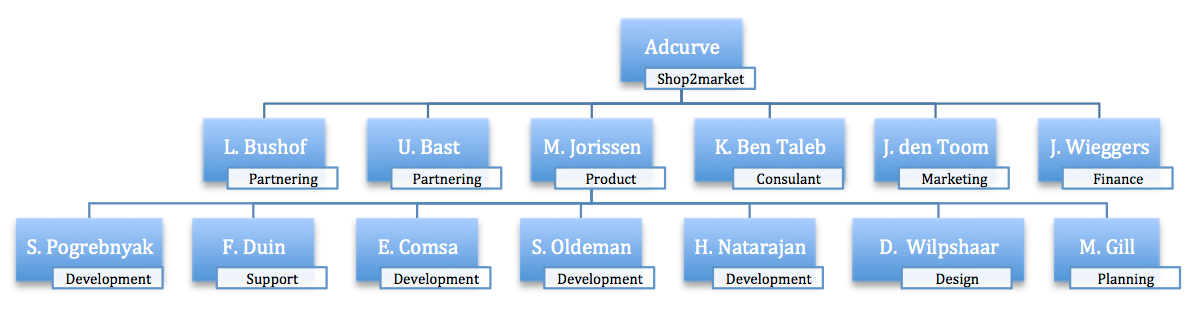
\includegraphics[width=0.9\textwidth]{organisation_structure.png}
    \caption{Organogram waarin het team en de relaties binnen Shop2market worden afgebeeld.}
    \label{fig:orgchart}
\end{figure}

\clearpage

\section{De kwestie} % een kwestie (aanleiding, het op te lossen probleem, de te vervullen behoefte of de te benutten kans);

Zoals te lezen valt in de aanleiding zijn er meerdere redenen voor dit project.

\begin{enumerate}
    \item Het kost momenteel te veel tijd om statistieken te berekenen. De berekeningen worden uitgevoerd met behulp van MongoDB MapReduce. Het team voorziet dat deze technologie niet genoeg schaalbaarheid biedt. Dit omdat rekentijd non-lineair is toegenomen in relatie tot de hoeveelheid data. Met de verwachte groei van Adcurve komen nieuwe eisen aan het licht en er moet naar een nieuwe oplossing worden gezocht.
    \item Bij voorkeur worden publishers geïntegreerd met behulp van API 's oftewel; een externe data bron. Op deze manier worden berekeningen uitgevoerd met precieze advertentiekosten. Maar doordat externe factoren nu een rol spelen in de berekeningen is het niet te garanderen dat de uitkomst altijd correct is. Zodra fouten intern of extern hersteld zijn, worden berekeningen voor een bepaalde dag, webwinkel of publisher opnieuw uitgevoerd. Het uitvoeren van dit soort correcties is tijdrovend door de huidige implementatie en gebruikte technieken.
    \item Webwinkels ontvangen tot soms tot 30 dagen na een bestelling een retournering van een of meerdere producten. Dit betekent dat een product niet verkocht is en de omzet uit de bestelling lager ligt dan is berekend. Het is wenselijk om berekende statistieken met betrekken tot retour bestellingen opnieuw te kunnen berekenen.
\end{enumerate}


\chapter{Project}
% de onderzoeksvragen, hoofdvraag met daaruit voortvloeiende deelvragen die moeten worden beantwoord

In \ref{sec:doelstelling} is de volgende doelstelling omschreven: ``Webwinkel eigenaren moeten in staat zijn om beslissingen te maken op basis van correcte en actuele gegevens in Adcurve. Dit betekent dat de gegevens die Adcurve toont altijd te verklaren zijn en overeenkomen met de werkelijkheid. De data moet op tijd verwerkt zijn, en fouten moeten tijdig hersteld kunnen worden.". 

Hieruit is een onderzoeksplan opgesteld. In het onderzoeksplan worden vijf deelvragen behandeld die samen de volgende hoofdvraag beantwoorden, namelijk:

{\large \textit{"Hoe verzorgt een nieuwe implementatie voor het up-to-date houden van statistieken in Adcurve zodat gegevens altijd te verklaren zijn?"}}
\medskip

\section{Onderzoeksvragen}

Om de hoofdvraag te beantwoorden zijn de volgende deelvragen geformuleerd

\begin{enumerate}
\item Wat zijn de functionele en niet functionele eisen waaraan de oplossing moet voldoen?
\item Wat zijn toonaangevende methodes en technologieën om statistieken te berekenen, die passen bij de wensen en eisen van de opdracht?
\item Wat zijn de probleemscenario's waardoor gegevens niet te verklaren zijn en wat zijn mogelijke oplossingen?
\item Wat zijn de mogelijke oplossingen en hoe wordt dit gevalideerd?
\item Wat zijn de gepresenteerde oplossingen en waarom zijn deze volledig of niet?
\end{enumerate}

\begin{comment}
\section{Literatuur} %  (optioneel) een beschrijving van de belangrijkste literatuur die onderzocht zal worden

Voorbeelden van mogelijk jargon die zullen voorkomen in de thesis zijn data aggregaties, data transformaties en het selecteren en installeren van big data tools. Deze concepten worden onderlegd door onder andere de volgende literatuur:

\begin{itemize}
    \item Data Mining, Concepts and Techniques \parencite{data-mining}
    \item I <3 Logs, Event data, stream processing, and data integration \parencite{logs}
    \item Fast Data Processing with Spark \parencite{spark}
    \item Real-Time Big Data Analytics \parencite{realtime-architectures}
\end{itemize}

Tijdens de selectie wordt mogelijk gebruik gemaakt van verschillende fases uit “de Berenschot-methode” \parencite{cuppen}.
Daarnaast zal tijdens het voeren van gesprekken, interviews en presentaties binnen de organisatie mogelijk gebruik worden gemaakt van de theorie uit “Adviseren als tweede beroep, resultaat bereiken als adviseur” \parencite{adviseren}.
\end{comment}

\newpage
\section{Onderzoek methode} % de te gebruiken methoden/technieken/middelen (ook van het onderzoek) en, indien van toepassing, de
\label{sec:onderzoekmethode}

% \section{Deelvragen} deelvragen voorkomend uit de gekozen ontwerpmethode (optioneel);

Voor kwalitatief onderzoek wordt een \textit{Case studie} gebruikt om de problemen in de gegeven context te analyseren. Methodes binnen dit type onderzoek zijn: explanatory, descriptive en exploratory. \parencite{john-dudovskiy}. Het onderzoek is ontworpen om de fases van een case studie uit te voeren. Het ontwerp is omschreven in tabel \ref{tab:onderzoekmethode}.

\begin{center}
\begin{table}[bh]
% \centering
\caption{Onderzoek methodes met te gebruiken methoden/technieken/middelen per deelvraag}
\label{tab:onderzoekmethode}
\def\arraystretch{1.5}
\begin{tabular}{|l|p{4cm}|p{2cm}|p{2.5cm}|p{4.5cm}|}

\hline
% \rowcolor{lightgray} 
\textbf{\#} & \textbf{Deelvraag} & \textbf{Type vraag} & \textbf{Methode} & \textbf{Actie / Resultaat} \\
\hline
1 & Wat zijn de functionele\newline en niet functionele eisen,\newline waaraan de oplossing\newline moet voldoen?
  & Descriptive
  & Interviews
  & MosCow prioriteiten lijst en checklist samenstellen \\
\hline
2 & Wat zijn toonaangevende\newline methodes en\newline technologieën om statistieken te berekenen, die passen bij de wensen en eisen van de opdracht?
  & Descriptive
  & Literature-\newline research
  & Analyseren van bronnen\newline m.b.v. van checklist wordt een shortlist samengesteld  \\
\hline
3 & Wat zijn de probleem\newline scenario's waardoor\newline gegevens niet te verklaren zijn en wat zijn mogelijke oplossingen?
  & Comparative
  & Interviews,\newline Literature-\newline research
  & Inventariseren op te lossen scenario 's\newline d.m.v. Impact analysis \\
  % 3a & Vergelijkingstabel huidige en wenselijke situatie met daarbij de technissche afhankelijkheden om een scenario te kunnen voorkomen \\
  % 3b & Door het toepassen van de vergelijkingstabel met gevonden technologieën worden mogelijke oplossingen ontworpen \\
\hline
4 & Wat zijn de mogelijke oplossingen en hoe wordt dit gevalideerd?
   & Designing
   & Literature-\newline research\newline group-\newline discussion
   & Door het Analyseren van\newline mogelijke ontwerpen en \newline groep- discussies worden\newline er POC 's\newline ontworpen met eisen. \\
\hline
5 & Wat zijn de gepresen-\newline teerde oplossingen\newline en waarom zijn deze\newline volledig of niet?
  & Explanatory
  & Case study
  & Conclusies op basis van verzamelde gegevens tijdens de proof of concept fase, zoals bijv. performance tests. Tabel van oplossingen met theorieën die het resultaat verklaren. \\
\hline
\end{tabular}
\end{table}
\end{center}

\clearpage

\section{Ethische overweging}

Zoals duidelijk wordt tijdens het onderzoek zijn er veel technologieën beschikbaar voor het verwerken van data. Om te voorkomen dat een oplossing wordt ontworpen op basis van de hype factor van een tool is er voor gekozen om een POC uit te voeren voor een kleine selectie aan technologieën.
Dit moet voorkomen dat een technologie in theorie wellicht de beste en de snelste is, maar uiteindelijk in een gegeven context niet werkt.

Met de rol van software engineer voelt de student zich mede verantwoordelijk voor het adequaat adviseren van stakeholders. Vanuit een Estische code is daarom overwogen om dieper onderzoek te doen naar de kernoorzaken achter de huidige probleemsituatie, zie \ref{sec:deelvraag3}.
Op de wijze wordt er ook op een objectieve wijze gekeken naar de situatie, om beslissingen tijdens het  project te valideren.

% Door het organiseren van groepsdiscussies wordt de organisatie betrokken in beslissingen.
Door het organiseren van groepsdiscussies wordt de inbreng vanuit de organisatie meegenomen. Zo is de student zich ervan bewust dat een gekozen technologie goed moet aansluiten bij de cultuur en kennis van de organisatie.

\clearpage


\chapter{Onderzoek}


% Deelvraag 1 ``Wat zijn de functionele en niet functionele eisen, waaraan de oplossing moet voldoen?"\ wordt beantwoord in \ref{sec:deelvraag1}

% Deelvraag 2 ``Wat zijn toonaangevende methodes en technologieën om statistieken te berekenen, die passen bij de wensen en eisen van de opdracht?"\  wordt beantwoord in \ref{sec:deelvraag2}

% MAIN QUESTION: "Hoe verzorgt een nieuwe implementatie voor het up-to-date houden van statistieken in Adcurve zodat gegevens altijd te verklaren zijn?"

In \ref{sec:deelvraag1} wordt gekeken naar ``Wat zijn de functionele en niet functionele eisen waaraan de oplossing moet voldoen?".

In \ref{sec:deelvraag2} wordt er gekeken naar ``Wat zijn toonaangevende methodes en technologieën om statistieken te berekenen, die passen bij de wensen en eisen van de opdracht?".


\clearpage

% ACTIVITY Afleggen interviews rondom Requirements \& Constraints, documenteren use-cases
% RESULT MosCow prioriteiten lijst en checklist
\section{Functionele en niet functionele eisen}
\label{sec:deelvraag1}

Wat zijn de functionele en niet functionele eisen, waaraan de oplossing moet voldoen?

In een interview met Matthijs Jorissen zijn de functionele en niet functionele eisen besproken. Vervolgens is hierin een prioriteit aangebracht met behulp van de MoSCoW methode. Hierbij worden alle project eisen in vier groepen ingedeeld: priority groups “MUST have”, “SHOULD have”, “COULD have”, en “WON’T have” \textcite{ma2009effectiveness}.

\begin{comment}
Een functionele eis kan gezien worden als iets dat de gebruiker nodig heeft om het doel te bereiken of een bepaalde voorwaarde waaraan de oplossing moet voldoen.

Een non functionele eis is een beperking doe wordt opgelegd op een mogelijke oplossing, met het doel om functionele eisen te behalen of het doel van het project.
\end{comment}

\begin{table}[bh]
\centering
\caption{lijst van eisen geprioritiseerd met behulp van de MoSCoW analyse}
\label{table:requirements}
\def\arraystretch{1.5}

\begin{tabular}{|l|p{12.5cm}|}
\hline
\textbf{Prioriteit} & \textbf{Functionaliteit/Requirement}
\\ \hline
Must have           & Statistieken voor één webwinkel kunnen opnieuw worden gegenereerd zodat veranderingen in externe data bronnen, bijvoorbeeld orders of geïmporteerde kosten, opnieuw worden geaggregeerd. Dit moet kunnen tot 30 dagen terug.
\\ \hline
Must have           & Het creëren van data aggregaties voor alle webwinkels over een dag, mag niet meer tijd in beslag nemen dan de huidige oplossing nodig heeft. Dit is 1 uur en 30 minuten.
\\ \hline
Must have           & De kosten voor eventuele licenties en infrastructuur mogen niet hoger zijn dan dat voor de huidige oplossing.
\\ \hline
Should have         & Statistieken zijn altijd voor kantoor uren beschikbaar voor het dashboard en voor latere processen zoals het genereren van tips.
\\ \hline
Should have         & De gekozen oplossing heeft een productief programmeermodel en is afhankelijk van hardware architectuur.
\\ \hline
Could have         & De programmatuur is testbaar en hierdoor eenvoudig te onderhouden.
\\ \hline
Could have          & Data aggregaties voor een groep webwinkels kunnen op een ander tijdstip worden geaggregeerd i.v.m. verschillende tijdszones.
\\ \hline
Could have         & De nieuwe oplossing moet schaalbaar zijn tot 10.000 webshops.
\\ \hline
\end{tabular}
\end{table}

Een aantal gebruikte termen zoals simpel, snel etc. worden verduidelijkt met de bijbehorende definities die in overleg tot stand zijn gekomen:

\begin{itemize}
    \item \textbf{Een productief programmeermodel} in de context van dit project wordt omschreven in \textcite{asanovic2006landscape}: "programming models should be independent of the number of processors, they should allow programmers to use a richer set of data types and sizes, and they should support successful and well-known parallel models of parallelism"

    \item \textbf{Scalability} wordt door \textcite{dubey2005recognition} gedefinieerd als: Schaalbaarheid is het vermogen om de gewenste snelheid te bieden en te onderhouden al dan niet verbeteren. De industrie heeft hier twee manieren voor. ``Scale up"\ is de methode waarbij hardware wordt vervangen zodat betere prestatie geleverd kan worden. Bij ``scale out"\ wordt er extra hardware aangesloten zodat een bestaand systeem de toenemende werkdruk kan ondersteunen.
\end{itemize}

\begin{comment}
TODO
\begin{itemize}
    \item Data aggregaties moeten plaatsvinden zodra kosten beschikbaar zijn per publisher
    
    \item voor probleem scenario 1 en 4, moet mogelijk zijn om voor een individuele webwinkels de data te aggregeren zodat er correcties kunnen worden gemaakt bij data kwaliteit issues. 
    \item de snelheid waarmee data wordt verwerkt moet snel genoeg zijn om 30 dagen aan data binnen 1 dag te verwerken.
    
    \item De tijd die het kost voor data aggregaties moet voorspelbaar zijn, dit kan worden bereikt wanneer de oplossing lineair schaalbaar is.
\end{itemize}

\end{comment}




\clearpage

% ACTIVITY Onderzoeken van toonaangevende, passende technologieën
\section{Toonaangevende methodes en technologieën}
\label{sec:deelvraag2}
Wat zijn toonaangevende methodes en technologieën om statistieken te berekenen, die passen bij de wensen en eisen van de opdracht?

Uit verschillende websites zijn voorbeelden van technologieën gevonden voor het verwerken van data, zie tabel \ref{tab:sites}. Sommige van de technologieën zijn bekend binnen de organisatie en in overleg met de opdrachtgever zijn een aantal richtingen geselecteerd om te onderzoeken, namelijk: databases, distributed systemen, en programmeer talen die optimaal gebruik maken van hardware performance.

\begin{table}[h]
\caption{Voorbeelden van mogelijke technologieën}
\label{tab:sites}
\def\arraystretch{1.5}
\begin{tabular}{|l|p{12.5cm}|}
\hline
\textbf{Voorbeelden} & \textbf{Website}                                                                 \\ \hline
Databases     & https://github.com/onurakpolat/awesome-bigdata                                     \\ \hline
Hadoop                                  & https://experfy.com/blog/hadoop-market-size-adoption-growth-2020/                  \\ \hline
Spark                                   & http://datanami.com/2014/11/21/spark-just-passed-hadoop-popularity-web-heres/      \\ \hline
Hardware                  & http://radar.oreilly.com/2014/01/a-compelling-family-of-dsls-for-data-science.html \\ \hline
\end{tabular}
\end{table}

De huidige oplossing maak gebruik van een MapReduce algoritme. Doordat de bestaande oplossing wordt getest met behulp van een nieuwe technologie zal dit worden meegenomen in het onderzoek. Er zijn eerdere vermeldingen gevonden van MapReduce onder een andere naam, Monte Carlo is omschreven door \textcite{asanovic2006landscape} en eerdere referenties zijn gevonden in \textcite{lee2010debunking}. In het onderzoek zal ook duidelijk komen hoe verschillende technologieën hier anders mee om gaan.

\newpage

\subsection{Database oplossingen}
\label{sec:databases}
Een mogelijke oplossing is om een Datawarehouse te implementeren waarin alle benodigde data bronnen worden beheerd en data aggregaties worden uitgevoerd.

Voor het maken van data aggregaties zijn basis SQL functies nodig: SUM, MIN, MAX, AVERAGE, samen met de SQL clauses: GROUP BY en HAVING. \parencite{data-mining}
Omdat bijna alle database systemen deze functies ondersteunen is er gekeken naar databases die een hoog volume aan data kunnen verwerken.

Veel Database Management Systemen (DBMS), ondersteunen de benodigde functies maar implementeren transactionele mechanismes om data integriteit te garanderen, bijvoorbeeld: ``locking-based concurrency control". Dit introduceert significante overhead. \parencite{harizopoulos2008oltp}. Verder raakt een DBMS overbelast wanneer een gevraagde opdracht\footnote{ Ieder SQL statement wordt vertaalt naar een opdracht door middel van een query plan.} niet optimaal kan worden uitgevoerd. Zo moet de opgevraagde dataset in het geheugen (RAM) passen, of er wordt terug gevallen op de harde schijf (zogeheten ``Disk spills"). De gegeven use-case vraagt om het frequent uitvoeren van aggregaties en corrigeren van data bronnen. De combinatie hiervan introduceert mogelijke performance problemen. \parencite{kersten2011researcher}
%"Moreover, database queries often contain blocking operations that lead to a pipeline stall or spilling large intermediates back to the disks." \parencite{kersten2011researcher}

% \footnote{Door frequent te aggregeren en corrigeren van data bronnen door middel van incremental loading of vervangen van datasets door 'UPDATE' of 'DELETE and INSERT' statements}
% Het plan in onze use-case is om frequent data aggregaties uit te voeren zodat statestieken in adcurve worden gecorrigeerd.

In vergelijking tot eerder genoemde OLTP (Online Transaction Processing) databases uit \textcite{kersten2011researcher} zijn er genoeg OLAP (Online Analytical Processing) systemen beschikbaar voor Data Warehouse toepassingen \parencite{data-mining}.

% In de paper "How To Build a High-Performance Data Warehouse" worden door de auteurs drie verschillende architectuur storage engines omschreven: Shared Memory, Shared Disk en Shared Nothing.

Michael Stonebraker, database pionier en origineel auteur PostgreSQL
\footnote{
 Opvallend is dat Bijna alle High Performance en Analytical databases afstammen van Postgres \parencite{postgresforks}. Dit dient als getuige van de enorme hoeveelheid research die is geïnvesteerd in (opensource) oplossingen op basis van PostgeSQL.
}
, omschrijft drie verschillende database storage engines: shared memory, shared disk en shared nothing. ``Because shared nothing does not typically have nearly as severe bus or resource contention as shared-memory or shared-disk machines, shared nothing can be made to scale to hundreds or even thousands of machines. Because of this, it is generally regarded as the best-scaling architecture". \parencite{dewitt2006build}


\subsubsection{\textbf{Conclusie}}

Er zijn verschillende beschikbare technologieën gevonden in de vorm een DBMS  Er zijn verschillende databases gevonden waarvan uit onderzoek blijkt dat de databases schaalbaar zijn in te zetten. De volgende databases zijn hieruit omschreven: Terradata, GreenplumDb, Vertica. Doordat deze databases niet gebruik maken van traditionele mechanismes en gebruik maken van een Shared Nothing architectuur zijn deze schaalbaar in te zetten. Dit is genoeg motivatie om een POC uit te voeren een van de databases, namelijk GreenplumDb. Dit omdat hier geen licentie kosten aan verbonden zijn.

\clearpage

\subsection{Distributed oplossingen}
\label{sec:distributed}
De indruk binnen de organisatie is dat de huidige oplossing niet schaalbaar genoeg is. Binnen distributed systemen wordt schaalbaarheid gerealiseerd door de ``scale out"\ methode.

% MapReduce wordt gezien als de oplossing wanneer de grootte van de dataesest niet effectief verwerkt kunnen worden door steeds groter groeiende databases. (TODO reference this)

HP Vertica, werd al eerder besproken in \ref{sec:databases}, en wordt omschreven als een ``distributed database to mean a sharednothing, scale-out system" \parencite{lamb2012vertica}. Hoewel alle MapReduce platformen hun performance behalen op zogeheten ``Commodity hardware"\ wordt bij databases ``Modern hardware"\ aanbevolen. Daarnaast zijn databases veelal commercieel waarbij Hadoop veel open source distributies kent. \parencite{dean2008mapreduce}

Hadoop staat bekend als de technologie met grote clusters, een voorbeeld van een distributed oplossing en een implementatie van Map Reduce, zo schrijft \textcite{hadoop2013selection}: ``The open-source software framework known as Apache Hadoop has gained sizable acceptance in organizations, spurred on by the growing digital business appetite for big data". Echter weten veel organisaties niet hoe ze deze technologie effectief moeten inzetten. Zo valt te concluderen uit \textcite{hadoop2015adoption} dat adoptie van het Hadoop ecosysteem nog altijd nog altijd laag blijft.

Afgezien van de adoptie blijft Hadoop interessant. Doordat de grootste bedrijven Hadoop blijven inzetten, met een groot aantal gebruikers, blijft het platform zich sterk ontwikkelen. In de loop der tijd zijn er SQL talen zoals Hive ontwikkeld waardoor het gebruikersgemak vele malen eenvoudiger is geworden. Echter introduceert dit nieuwe uitdagingen. Doordat data sets frequenter worden opgevraagd is er mogelijke terugval in performance\footnote{Lees: adhoc query 's vs. reporting query 's}. \parencite{thusoo2010hive}

Daarnaast blijkt uit benchmarks door \textcite{armbrust2015spark} dat Spark SQL competitief is met vergelijkbare SQL talen op Hadoop zoals Hive en Impala\footnote{Impala en Hive worden aangeboden, afhankelijk van de Hadoop distributie. De performance is vergelijkbaar afhankelijk van de configuratie en hoeveelheid query 's. \parencite{hortonworks_benchmark}}.

Apache Spark, origineel ontwikkeld in UC Berkley heeft sinds zijn release in 2014 als open source project meer contributies gezien dan Apache Hadoop in totaal heeft ontvangen\footnote{Met over 400 contributies is Apache Spark het meest actieve data processing framework in de industrie}. \parencite{armbrust2015spark}. Dit is veelbelovend en ook vanuit Shop2market is er een enorme interesse. In 2015 zijn er al succesvolle experimenten uitgevoerd met SparkML voor een Machine Learning applicatie.

\subsubsection{\textbf{Conclusie}}

Er zijn verschillende technologieën gevonden die gebruik maken van een distributed of networked methode. Omdat in de huidige situatie de data sets niet groter zijn dan 2GB wordt er voor gekozen om geen POC uit te voeren met Hadoop.  In eerdere ervaring met Hive duren gegeven opdrachten minimaal tussen de 15 en 17 minuten. Dit is te verklaren doordat de SQL query 's worden vertaald naar de onderliggende MapReduce fases. \parencite{thusoo2010hive} Dit introduceert een significante overhead voor de huidige use case.

Daarnaast is gevonden dat Spark SQL deze overhead niet ervaart doordat alle data communicatie in-memory plaats vindt. In tegendeel tot de verschillende fases in Hadoop waarbij er wordt gelezen en geschreven van het filesysteem (HDFS). Dit is genoeg motivatie om een POC uit te voeren met Apache Spark
% waarbij Spark een vergelijkbaar algoritme toepast met dat van MapReduce maar veel performance gerelateerde issues voorkomen kunnen worden door het gebruik van in-memory data communicatie tussen verschillende fases.
% \verb TODO: add citation ``Comparing Apache Spark and Map Reduce with Performance Analysis using K-Means"

\clearpage

\subsection{Hardware oplossingen}
\label{sec:hardware}
Een van de oplossingen die wordt onderzocht is het gebruik maken van krachtige hardware componenten (zowel de CPU en de GPU). Dit is mogelijk met expert talen zoals; Verilog, CUDA of OpenCL of C++.


Op de universiteit van Stanford is hier veel onderzoek naar gedaan. Dit vereist alleen veel hardware specifieke kennis en moet in code worden uitgedrukt: "programming these devices to run efficiently and correctly is difficult, error-prone, and results in software that is harder to read and maintain." \parencite{sujeeth2011optiml}. Daarom is er een serie aan DSL's ontwikkeld\footnote{Voorbeelden van DLS 's zijn \TeX, HTML en SQL  \parencite{sigplan2000dsl}}

Terwijl \textcite{sujeeth2011optiml} een veelbelovende oplossing lijkt aan te bieden is het project nog altijd in Alpha versie \parencite{optiml_project_home}. Hetzelfde team presenteerde in 2014 Forge, een DSL voor expert talen met veelbelovende test resultaten: "Forge-generated Delite DSLs perform within 2x of hand-optimized C++ and up to 40x better than Spark" \parencite{sujeeth2014forge}. Helaas lijkt hierbij hetzelfde probleem te spelen en is er niet genoeg documentatie gevonden om hier een POC mee te starten.

Binnen Shop2market zijn veel performance gerelateerde projecten opgelost met Golang. Naast dat dit erg productief is bevonden biedt de moderne taal een alternatief concurrency model. "C, C++, and to some extent Java are quite old, designed before the advent of multicore machines, networking, and web application development. There are features of the modern world that are better met by newer approaches, such as built-in concurrency." \parencite{pike2012go}.

\subsubsection{\textbf{Conclusie}}

De besproken technologieën zijn de DSL talen: OptiML, OptiSQL en Forge. Bij gebrek aan praktische voorbeelden en algemene documentatie is er voor gekozen om hier niet verder in te investeren. Er zou niet voldoende kennis zijn om een mogelijke POC naar productie te brengen. Hoewel Forge tijdens de benchmarks extreem goed presteert, wordt niet vermeld welke algoritmes hierbij zijn gebruikt. Omdat in de huidige implementatie gebruik wordt maakt van MapReduce (de Monte Carlo methode) hoeft deze performance niet behaalt te worden. Zo schrijft \textcite{lee2010debunking}: "Monte Carlo algorithms are generally compute-bound with regular access patterns, which makes it a very good fit for SIMD architectures", in vergelijking met een GPU processor. Golang biedt hier een mogelijke oplossing, omdat de taal een productieve manier biedt om optimaal gebruik te maken van Multicore CPU's.

\clearpage

\section{Conclusies}
\label{sec:gevonden_tools}
Uit de verschillende oplossingsrichtingen zijn een aantal technologieën onderzocht in sectie \ref{sec:deelvraag2} t/m \ref{sec:hardware}. Deze zijn besproken in een groepsdiscussie waarbij de volgende non functionele eisen worden getoetst. Hiervoor is een checklist samengesteld, gebaseerd op de projecteisen omschreven in \ref{sec:deelvraag1}, en aanvullende eisen (1 en 5) die ter spraken zijn gekomen tijdens de discussie. Per vergelijkingsmatrix is af te lezen hoe iedere technologie scoort tegenover de volgende checklist in figuur \ref{tab:checklist}.

\begin{table}[h]
\centering
\caption{Checklist met criteria gebruikt in vergelijkingsmatrix}
\label{tab:checklist}
\def\arraystretch{1.2}
\begin{tabular}{l|p{11cm}c}
label       & criteria                                                          & zwaarte \\ \hline
support     & genoeg ondersteuning vanuit open source of commerciële industrie; & 3       \\
scalability & indicatoren tot schaalbaarheid en high performance;               & 2       \\
productief  & ondersteund een productief programmeer model;                     & 2       \\
testbaar    & code is testbaar door middel van unit tests.                      & 1       \\
kennis      & er is genoeg kennis beschikbaar binnen of buiten de organisatie   & 1      
\end{tabular}
\end{table}

\subsubsection{\textbf{Database oplossingen}}

In vergelijkingsmatrix \ref{tab:matrix_databases} wordt duidelijk dat de database slecht worden beoordeeld op het gebied van testbaarheid en kennis. Er is hiervoor niet genoeg ondersteuning binnen de organisatie om gebruik te maken van een database oplossing. De grootste zorg is de kans dat toenemende complexiteit van SQL queries en het gebrek aan expert kennis voor problemen zorgt.

\begin{table}[bh]
\caption{Vergelijkingsmatrix waarin eisen worden getoetst tegenover de gevonden databases}
\label{tab:matrix_databases}
\begin{tabular}{|p{3cm}|l|l|l|l|l|l|}
\hline
           & support & scalability               & productief & testbaar & kennis &     (score)  \\ \hline
GreenplumDB & +       & +                         & -          & -        & -      & 5     \\ \hline
Vertica     & +       & +                         & +          & -        & -      & 7     \\ \hline
Redshift    & +       & +                         & +          & -        & -      & 7     \\ \hline
\end{tabular}
\end{table}

\subsubsection{\textbf{Distributed oplossingen}}

In vergelijkingsmatrix \ref{tab:matrix_distributed} wordt duidelijk dat de distributed oplossingen slecht worden beoordeeld op het gebied productiviteit. De voornaamste verklaring hiervoor is ook naar voren gekomen in het onderzoek \ref{sec:distributed}. De tijd die een MapReduce job in beslag neemt is onvoorspelbaar bij adhoc queries. Dit kan betekenen dat het lang duurt voordat een developer feedback krijgt tijdens het ontwikkelen. In tegenstelling is dit geen probleem bij Spark omdat een cluster in standalone-mode op een locale laptop kan worden gestart. Daarom scoort Spark veel hoger. Over het testen van implementaties in Spark valt nog te onderzoeken. Daarnaast is het een afweging waard om code te implementeren in Python, maar uit onderzoek blijkt een implementatie in Spark SQL 10x sneller te zijn door een optimale vertaling van SQL \parencite{armbrust2015spark}.

\begin{table}[bh]
\caption{Vergelijkingsmatrix waarin eisen worden getoetst tegenover de gevonden distributed systemen}
\label{tab:matrix_distributed}
\begin{tabular}{|p{3cm}|l|l|l|l|l|l|}
\hline
                & support & scalability               & productief & testbaar & kennis &     (score)  \\ \hline
Hadoop / Hive   & +       & +                         & -          & -        & +      & 6     \\ \hline
Hadoop / Python & +       & +                         & -          & +        & +      & 7     \\ \hline
Spark SQL       & +       & +                         & +          & -        & +      & 8     \\ \hline
Spark / Python  & +       & +                        & +          & +        & +      & 8     \\ \hline
\end{tabular}
\end{table}

\clearpage

\subsubsection{\textbf{Hardware oplossingen}}

In vergelijkingsmatrix \ref{tab:matrix_hardware} wordt duidelijk dat deze programmeer talen indicatoren hebben om hoge performance te bereiken. Tijdens het onderzoek in \ref{sec:hardware} zijn er veel expert talen besproken. In vergelijkingsmatrix zijn slechts een aantal van deze talen opgenomen ter referentie, namelijk Verilog en C++ en zijn al eerder besproken als minder productief. Het onderwerp scalability moet anders worden geinterperteerd in dit geval, omdat er geen sprake is van een dataprocessing tool. Toch is de consensus dat deze talen de mogelijkheid bieden om hoge performance te behalen. Met behulp van een up-scaling methode of out-scaling door het inzetten van de aanwezige architectuur met Resqueue. Op deze manier kun data bijvoorbeeld per webshop worden verwerkt over verschillende machines, vergelijkbaar met MapReduce. De testbaarheid van programmeer talen is erg goed beoordeeld. Als laatste zijn de onderzochte DSL talen OptiSQL en Forge slecht beoordeeld door het gebrek aan beschikbare informatie, kennis en documentatie.

\begin{table}[bh]
\caption{Vergelijkingsmatrix waarin eisen worden getoetst tegenover de gevonden programmeer talen}
\label{tab:matrix_hardware}
\begin{tabular}{|p{3cm}|l|l|l|l|l|l|}
\hline
           & support & scalability               & productief & testbaar & kennis &     (score)  \\ \hline
Verilog    & -       & +                         & -          & -        & -      & 2     \\ \hline
C++        & +       & +                         & -          & -        & +      & 6     \\ \hline
OptiSQL    & -       & +                         & +          & +        & -      & 5     \\ \hline
Forge      & -       & +                         & +          & +        & -      & 5     \\ \hline
Golang     & +       & +                         & +          & +        & +      & 8     \\ \hline
\end{tabular}
\end{table}

\subsubsection{\textbf{Conclusie}}

Alle omschreven gevonden technologieën in Deelvraag 2 zijn beoordeeld. Hiermee wordt de volgende vraag beantwoord: ``Wat zijn toonaangevende methodes en technologieën om statistieken te berekenen, die passen bij de wensen en eisen van de opdracht?". Voor de beoordeling is onderzoek gedaan te lezen in hoofdstuk \ref{sec:deelvraag2}. Vervolgens zijn alle omschreven technologieën beoordeeld door middel van de checklist (zie tabel \ref{tab:checklist}) en aan de hand van groupsdiscussies.

Hieruit is gekomen dat Golang en Spark met een 8 zijn beoordeeld, daarna de databases Vertica en Redshift met een 7. Omdat er niet genoeg consensus is over het toepassen van een database oplossingen wordt deze niet getest. Dit betekend dat Golang en Spark worden getest in een tweetal Proof of Concept 's.


\chapter{Resultaat}

In \ref{sec:deelvraag3} wordt gekeken naar ``Wat zijn de probleem scenario 's waardoor gegevens niet te verklaren zijn, en wat zijn de mogelijke oplossingen?".

In \ref{sec:deelvraag4} wordt er gekeken naar ``Wat zijn de mogelijke oplossingen en hoe wordt dit gevalideerd?".

In \ref{sec:deelvraag5} is te lezen hoe deelvraag 5 wordt beantwoord, ``Wat zijn de gepresenteerde oplossingen en waarom zijn deze volledig of niet?".

\clearpage


% ACTIVITY Impact analyse uitvoeren rondom use-cases
\section{Problematische scenario 's en mogelijke oplossingen}
\label{sec:deelvraag3}
\textit{Wat zijn de probleem scenario's waardoor gegevens niet te verklaren zijn, en wat zijn de mogelijke oplossingen?}

Tijdens de project analyse is met verschillende stakeholders binnen de organisatie gesproken. Naast de gedefinieerde projecteisen zijn er verschillende symptomen verzameld. Deze zijn gebruikt voor het samenstellen van een Impact analyse gemaakt, zie Apendix \ref{app:impact_analyse}

Vervolgens is per probleemscenario een mogelijke technische verklaring gezocht, zijn er criteria omschreven waaraan de gebruikte technologie bij een mogelijk oplossing moet voldoen. Hierdoor wordt getoetst of de geselecteerde technologieën in \ref{sec:gevonden_tools} toepasbaar zijn en de huidige probleem scenario werkelijk kunnen oplossen.

\subsection{Scenario's uit de Impact Analyse}

\begin{enumerate}
    \item L6: API 's provided by the publisher are unavailable
    \item M5: API 's for google, change frequently and the import stops working, or fail silent (values are not matched,,resulting in empty fields)
    \item H6: Wrong costs by configuration, issues: mistakes in tracking Order amount, tracked wrong, multiplied by 100 bug
    \item L7: Metrics calculated incorrectly because of mismatching product data (ids from tracking don't match cost exports from publisher)
    \item L7: Calculations fail,because technology or infrastructure 
    \item L4: Aggregations from different dimensions on the same data
    don't match
    \item H7 Bij het bekijken van dashboards in Adcurve zijn de gegevens over de vorige dag pas beschikbaar na 12:30 CET. Omdat alle data in een keer wordt verwerkt wordt het proces gestart nadat alle afhankelijke data bronnen beschikbaar zijn.
\end{enumerate}

Scenario een (1) tot en met vier (4) zijn niet te voorkomen omdat de organisatie zelf hier weinig invloed op kan hebben. Het wordt veroorzaakt door externe processen bij publishers, of mensen in diesnt van de webwinkel die de advertenties of webwinkel integraties verkeerd configureren. Scenario vijf (5) en zes (6) hebben een hoge impact en zijn specifieke problemen met de huidige implementatie. Deze scenario's zijn te voorkomen door het inzetten van andere technologie of een andere strategie als het aan komt op data processing.
Scenario 7 is eerder besproken tijdens de non functionele eisen in \ref{table:requirements}. Deze is opgenomen zodat onderzocht wordt hoe dit het best kan worden voorkomen.  

\clearpage

\subsection{Technische te verklaren oorzaken}

Met betrekking tot scenario vijf (5) en zeven (6) zijn verschillende problemen gevonden in relatie tot de gebruikte versie van MongoDB \parencite{mongo_changelog}. Uit monitoring systemen zijn de foutmeldingen terug te relateren aan software bugs die aanwezige zijn in versie 2.4.

De consensus binnen de organisatie is dat een upgrade naar een volgende versie riskant is. Het is niet in te schatten hoe veel problemen er zullen optreden. Daarnaast moeten er processen worden ingericht om het synchroniseren van order te ondersteunen en data verlies te voorkomen wanneer de database offline moet.
% TODO: is het mogelijke om machines van verschillende versies naast elkaar te draaien in een cluster?
    
Met betrekking tot scenario zeven (7) zijn de volgende mogelijke oorzaken gevonden:

\begin{itemize}
    \item Uit monitoring systemen blijkt dat het online productie processen van invloed zijn op de performance van het aggregatie proces. Omdat MongoDB direct wordt gebruikt voor het synchroniseren van bestellingen met webwinkels, en dit een realtime proces is, wordt het cluster hiermee belast. In de huidige situatie worden de MapReduce jobs op een aantal machines in het cluster uitgevoerd, toch word de performance beïnvloed.
    \item het aggregeren van data kan in MongoDB wellicht trager zijn dan nodig omdat de tussentijdse resultaten uit de fases in MapReduce worden weggeschreven naar verschillende machines \parencite{mongo_mr_shards}. Zo valt ook af te lezen uit monitoring dat het wegschrijven van de uiteindelijk resultaten langer duurt dan het aggregeren zelf. Dit heeft mogelijk te maken met het bijhouden van indexes.  \parencite{mongo_write_performance}
    % replica sets? sharding? grootte cluster?
\end{itemize}


\subsubsection{\textbf{Conclusie}}
\label{subsec:3.3.2}

Tijdens de root cause analysis zijn een aantal oorzaken omschreven. Hieruit valt te concluderen dat een mogelijke nieuwe oplossing aan de volgende criteria moet voldoen:

\begin{enumerate}[label=(\alph*)]

    % Er rekening moet worden gehouden met de mogelijke overhead van networking applications, en tegelijkertijd de mogelijkheid moet zijn om grootte data sets op te splitsen zodat er geen ``disk spills"\ optreden.
    \item In de nieuwe situatie moet op efficiënte wijze worden om gegaan met een kleine hoeveelheid aan data, zodat de verschillende fases van het aggregeren (zoals map, reduce, shuffle en sort). Dit omdat voor 80\% van de webshops een kleine hoeveelheid data wordt verzameld. Tegelijkertijd is de input data set groot en zijn resultaten van aggregaties wellicht groter. Er moet in deze situatie op efficiënte wijze data worden weg geschreven naar een eindlocatie,  zoals het filesysteem. Hierbij moet het onderhouden van indexes worden voorkomen.
    
    \item Er moet situaties situatie worden voorkomen waarin het onmogelijk is om een technologie of systeem te upgraden naar een nieuwere versie. Dit is te voorkomen door a) geen state te bewaren in het systeem zelf, maar dit alleen te gebruiken bij data processing. b) door het systeem onafhankelijk te maken van productie / online processen. Dit biedt de mogelijkheid door bijvoorbeeld een database back-up te doen, het systeem te migreren en de data opnieuw in te laden.
\end{enumerate}

\clearpage


\subsection{Hoe wordt dit voorkomen met de gevonden tools / POC?}
\label{subsec:deelvraag3_vergelijking}


\subsubsection{\textbf{Versie upgrades}}

Door de tools binnen het Hadoop ecosysteem wordt geen state bewaard. Maar alle data wordt beheerd door HDFS en opgeslagen als toegankelijke bestanden in een gekozen bestandsformaat. Het risico is dat het upgraden van versies, niet compatible met verschillende bestands formaten. Ook de tools die opereren op het data formaat moeten compatible zij. Daarnaast bestaat de mogelijkheid dat HDFS data anders beheerd onder verschillende versies. Hierdoor zijn data migraties erg operationeel intensief is. Hierdoor is het sterk aan te raden om dit niet zelf te beheren, maar gebruik te maken van distributie zoals Amazon EMR, Hortonworks, Cloudera of MapR.

Omdat Spark onder andere uitmaakt van het Hadoop ecosysteem zijn deze conclusies te generaliseren.

Omdat databases bij definitie statefull zijn, moet er in dit geval een back-up en restore mogelijkheid aanwezig zijn om upgrades te kunnen uitvoeren.

In het geval van Golang, dat in het algemeen niet als data processing tool te beschouwen is maar als een General purpose language, is de implementatie code eenvoudig te upgraden naar nieuwere versies. Dit wordt gegarandeerd als de implementatie volledig getest is door unit tests. 


\subsubsection{\textbf{Mogelijke overhead voorkomen}}

\begin{verbatim}

Use the COST PAPER (single threading vs. network overhead)

https://www.usenix.org/conference/hotos15/workshop-program/presentation/mcsherry

AND The paper measuring NETWORK OPTIMIZATIONS vs CPU/MEM in DATA PROCESSING TOOLS VS CPU
https://www.usenix.org/system/files/conference/nsdi15/nsdi15-paper-ousterhout.pdf

Reference to the paper and explain:
SPARK USES NO INDEX \parencite{armbrust2015spark}
MAP REDUCE (Google / Apache) USES NO INDEX 
SHARED NOTHING DATABASES USE NO INDEXES \parencite{lamb2012vertica} of \parencite{harizopoulos2008oltp} / \parencite{dewitt2006build}

MAYBE ALSO APPLY 'Amdahls law'
https://en.wikipedia.org/wiki/Amdahl%27s_law

 AND MAYBE 
"roughly 80\% of the effects come from 20\%"
https://en.wikipedia.org/wiki/Pareto_principle

\end{verbatim}


\subsubsection{\textbf{Oplosing om  high query speed en good analytics performance te behalen met  twee losse systemen}}

Het splitsen van data verwerken en data opslag / opvragen betekend dat de geaggregeerde data zal worden opgeslagen in s3, zodat de bestaande API de data kan uitserveren. 
De aggregaties op basis van week, jaar en maand komen te vervallen. De overige aggregatie die nodig is om API client snel te houden wordt gedaan door Saki. Doordat de bestanden gesorteerd worden opgeslagen op s3, kan saki deze binnen 100 milliseconden aggregeren per query.

Dit heeft als gevolg dat data opslag volledig verplaatst naar Amazon S3, zowel de input data als de output data. (data pipeline)

    
\subsection{Conclusie}

Een deel van het probleem is het actief monitoren van de data kwaliteit en processen starten om het te corrigeren. Hier wordt niet verder op in gegaan omdat een dergelijke oplossing hiervoor buiten scope valt. Hiervoor geldt, zodra er een oplossing is moeten de datakwaliteit worden herstelt door het proces te starten dat de correcties uitvoert [``effected datasources"\ opnieuw evalueren]
Deze scenario's zijn ook tegelijkertijd lastig te voorkomen, alleen te herstellen. Het advies is daarom om hier ``monitoring en alerting\ voor te implementeren en verder onderzoek doen naar bestaande methodieken voor beheersen van datakwaliteit. Bijvoorbeeld door starten van een ``Data Stewardship Program" zoals omschreven wordt in het ``TDWI Report, The Data Warehouse Institute"\ door  \textcite{eckerson2002data}.

Spark SQL is bewezen snel erg snel te zijn en Amazon EMR is managed service

database column store heeft geen indexes maar partities, bewezen erg snel te zijn… maar geen voordelen worden behaald omdat  ons proces altijd N-max aantal columns worden opgevraagd. Daarom zal de query nooit sneller zijn, unless er meerdere query 's zijn waarbij verschillende columnen worden opgevraagd. Daarom zijn er te weinig voordelen om hier een POC mee te starten, daarnaast zullen versie upgrades lastig zijn. 

De Aggregatie processen met Golang zullen erg klein worden gemaakt door de data van te voren te partitioneren per shop. Dit biedt de mogelijkheid om het deze processen uit te voeren op verschillende machines (scale-out), door het gebruikt van resqueue workers "Resque workers can be distributed between multiple machines, support priorities, are resilient to memory bloat / "leaks," \parencite{github2016reque} 


Kort: Er wordt niet verder geïnvesteerd in een POC met databases omdat er te veel keuze is, en technologie niet effectief is toe te passen

Wel wordt er een POC uitgevoerd met Golang en Spark


% Het splitsen van data verwerken en een databases waaruit de data is op te vragen, heeft met gevolg dat Saki, een applicatie die in real time aggregaties op het hoogste niveau pakt (channel, shop, shop_product_id) en deze flexibel aggregeerd op basis van datum.
\clearpage

% ACTIVITY Bespreken van ontwerpen en evt. aanpassen van ontwerpen
% ACTIVITY Vastleggen kwaliteitscriteria Proof of concept's
\section{Ontworpen experimenten middels proof of concept}
\label{sec:deelvraag4}
% \textbf{Hardware oplossing met Golang}
% Het is praktisch mogelijk om data in sub sets te aggregeren omdat er een afzonderlijke data bron is per publisher.
% Het gebruiken van gesplitste bestanden per webshop zorgt voor zeer korte levende processen. De totale performance hoeft niet te verbeteren, zolang het proces dat alleen data aggregatie uitvoert voor de specifieke webwinkel en publisher kort van duur is kan dit worden uitgevoerd op verschillende machines tegelijk om dit schaalbaar in te zetten. "We typically find that the highest performance is achieved when multiple threads are used per core. For Core i7, the best performance comes from running 8 threads on 4 cores" \parencite{lee2010debunking}

% \textbf{Distributed oplossing met Spark}
% Door gebruik te maken van distributed functionaliteiten van Spark wordt getest of de snelheid waar spark bekend om staat (paper) behaald kan worden in onze use case. Er is de mogelijkheid om unit tests en functional tests te schrijven, dit wordt aangeboden door het framework. Het wegschrijven van meerdere resultaten in een proces kan door het partitionener van output data op (PublisherID, ShopID). Ook kunnen er meerdere dagen in een proces worden verwerkt en het resultaat wordt weggeschreven per TimeID, PublisherID en ShopID


In dit hoofdstuk wordt omschreven hoe de Proof of concept 's zijn ontworpen. Zoals is te lezen in \ref{sec:deelvraag3} zijn de best mogelijke oplossingen te ontwikkelen met behulp van \textit{Golang} en \textit{Apache Spark}. In overeenstemming met de organisatie zijn verdere succesfactoren gedefinieerd per POC.


% De uitvoer van het project bestaat uit drie fases; Data preperation, Go Aggregate en Spark SQL
% In fase 1 vindt de ETl processing plaats. Als de resultaten snel genoeg zijn, zal dit worden hergebruikt in fase 2 en 3.
% TODO Leg uit dat Spark SQL niet wordt aangeraden voor ETL wanneer dit alleen mapping fases heeft


\subsection{Ontworpen experimenten}

Zoals wordt omschreven in de originele doelstelling in \ref{sec:doelstelling} ``moet data op tijd worden verwerkt evenals het tijdig herstellen van fouten mogelijk zijn".  Daarom valideert dit experiment welke oplossing de beste prestatie levert in de huidige situatie. Voor het meten van performance worden er drie verschillende type aggregaties uitgevoerd op "commodity hardware", de exacte specificaties worden later omschreven in sectie \ref{subsec:hardware_specs}.  Er wordt gebruik gemaakt van een productie data set van één willekeurige dag.

Tijdens iedere aggregatie worden er twee metingen uitgevoerd: de totale proces tijd \footnote{tijd word gemeten door unix `time` zie de documentatie voor time: \url{http://linux.die.net/man/1/time}} en de  tijd zonder ``warmup time".  Warmup time wordt in dit experiment omschreven als de tijd tussen het starten van het proces en het werkelijk uitvoeren van de geschreven implementatie. Voor het evalueren van de twee POC 's is besloten om geen latency, IO, memory of CPU gerelateerde benchmarks te evalueren. Dit is wel gewoonlijk bij \textbf{industrie benchmarks} van verschillende data processing tools. Maar dit wordt gedaan vanuit een competitief perspectief  \parencite{ousterhout2015making}. Voor de doelstellingen van dit project is de totale proces tijd belangrijker.

\subsection{Gebruikte data sets}

Tijdens de drie fases van het experiment wordt gebruik gemaakt van een data set uit productie als data input. De data set bestaat uit visits en orders van 264 webwinkels.

\begin{itemize}
    \item Het \textbf{orders} bestand is origineel 0.2494 GB (249.0 MB) groot, dit is in een Binary JSON (BSON) compressie formaat, Na het ETL waarbij alleen de alleen de relevantie metrieke overblijven is de dataset 0.04734 GB (5.0 MB) groot. Dit is een JSON formaat waarbij alle extra kolommen voor visits ook zijn inbegrepen en een default waarde hebben.

    \item Het \textbf{visits} bestand is origineel 1.0GB groot, dit is in een CSV bestand waarbij de TAB charachter als delimiter wordt gebruikt.  Na het ETL waarbij alleen de alleen de relevantie metrieken overblijven is de dataset 0.04734 GB groot. Dit is hetzelfde JSON formaat waarbij alle extra kolommen voor orders zijn inbegrepen en een default waarde hebben.
\end{itemize}

Het resultaat van de ETL voor orders en visits wordt als input data gebruikt voor iedere aggregatie. De drie aggregaties zijn variaties waarbij dezelfde input data wordt gebruikt, maar waarvan het resultaat verschilt per aggregatie in data grootte. Dit is om de huidige situatie en business needs te simuleren. Een grotere data set past wellicht wel of niet in het geheugen (RAM). De drie variaties maken gebruik van de volgende keys waarop de aggregatie functie \verb=SUM(metric)= wordt toegepast:

\begin{itemize}
    \item TimeId, ChannelID
    \item TimeId, ChannelID, ShopId
    \item TimeId, ChannelID, ShopId, ShopProductId
\end{itemize}

Ieder opdracht (aggregatie) wordt in één serie vijf keer herhaalt, waarvan een vervolgens de twee metingen worden geregistreerd. Over de metingen wordt een gemiddelde genomen voor het resultaat.

\subsection{Gebruikte Hardware}
\label{subsec:hardware_specs}

Tijdens het onderzoek naar verschillende technologiën zijn ook benchmarks gevonden. Hierbij wordt er vaak gepretendeert dat er een schaalbaarheid kan worden bereikt door het gebruiken van "Commodity hardware". Hiermee worden machines bedoelt die algemeen beschikbaar zijn, geen bijzondere performance voordelen bieden. Om in deze trend te blijven is er voor gekozen om geen speciale omgeving te installeren voor de experimenten. Uiteindelijk is er gebruik gemaakt van een Macbook Pro met de volgende specificaties:

\begin{table}[h]
\caption{Hardware specificaties van de gebruikte machine}
\label{tab:hardware_specs}
\begin{tabular}{ll}
Merk:      & MacBook Pro (Retina, 13-inch, Mid 2014) \\
Processor: & 2.6 GHz Intel Core i5                   \\
Geheugen:  & 8 GB 1600 MHz DDR3                      \\
Storage:   & Apple SSD                                  
\end{tabular}
\end{table}

\subsection{ETL Process, Data preparation}

Het proces dat voorziet in de eerste fase van het proces is geschreven in Golang. Hier zal voor de rest van het document naar worden gerefereerd als de splitter. ETL (Extract, Transform and Load) is een manier om data uit een externe databron te transformeren naar een ander schema   \parencite{data-mining}. Dit zorgt voor een uniform of formaat waardoor latere processen geen logica hoeven toe te passen om met de data te werken. In deze context worden er alleen met bestanden gewerkt, de dataflow gaat als volgt:

\begin{enumerate}
    \item Extract / download bestanden van Amazon S3
    \item Transform / bewerk de bestanden op locale hardeschijf met de splitter implementatie in Golang waardoor een BSON of CSV formaat wordt omgezet naar JSON met een uniform schema.
    \item Load / het resultaat wordt weg geschreven naar de locale hardeschijf. In het ontwerp is er voor gekozen om data te partitioneren per \verb+shop_id+ voor later gebruik.
\end{enumerate}

Ter illustratie is in tabel \ref{tab:etl_input_example} worden een aantal kolommen uit de input data gebruikt, in dit geval uit de CSV met visits. Iedere regel in dit bestand representeert een bezoek op de website van een webshop. Deze bezoeken komen voort uit advertenties die door Adcurve zijn gepubliceerd bij de publishers.

\begin{table}[bh]
\centering
\caption{Een voorbeeld van de input data gebruikt tijdens ETL}
\label{tab:etl_input_example}
\begin{tabular}{|l|l|l|l|l|l|}
\hline
timestamp  & time\_id & publisher\_id & shop\_id & shop\_product\_id & shop\_category\_id \\ \hline
1464154281 & 20160424 & 410         & 224      & 103774145         & 338790             \\ \hline
1464154306 & 20160424 & 61          & 910      & 108837485         & 6782117            \\ \hline
1464154314 & 20160424 & 410         & 224      & 100670758         & 9152995            \\ \hline
\end{tabular}
\end{table}

Zoals te zien is in figuur \ref{fig:visits.json_after_etl} wordt iedere regel uit het CSV bestand getransformeerd naar het JSON formaat. Daarnaast wordt er een extra kolom toegevoegd: \verb+Traffic=1+, naast de andere kollomen die dienen als ``placeholders"\ voor de orders data. Dit is een bewuste keuze in het ontwerp voor het behalen van mogelijke betere performance. Dit komt ook ten goede van de data consistentie omdat de data interpretatie van data in één fase plaatsvindt. De vervolg fases kunnen hierdoor gebruik maken van pure functies die in een framework, technologie of taal zijn geïmplementeerd.

\begin{figure}[htb]
% \centering
\caption{De bestanden en hun formaat na het ETL proces door de Splitter}
\label{fig:visits.json_after_etl}
\begin{verbatim}
/Users/stefano/dev/go-aggregate/exports/224/visits.json
{"TimeId":"20160424","OrderID":"","ShopID":224,"ChannelID":410,
"ShopProductID":103774145,"ShopCategoryID":338790,"Traffic":1,
 "Order":0,"Amount":0,"ExAmount":0,"Cost":0}\n
{"TimeId":"20160424","OrderID":"","ShopID":224,"ChannelID":410,
 "ShopProductID":100670758,"ShopCategoryID":9152995,"Traffic":1,
 "Order":0,"Amount":0,"ExAmount":0,"Cost":0}\%
    
/Users/stefano/dev/go-aggregate/exports/910/visits.json
{"TimeId":"20160424","OrderID":"","ShopID":910,"ChannelID":61,
 "ShopProductID":108837485,"ShopCategoryID":6782117,"Traffic":1,
 "Order":0,"Amount":0,"ExAmount":0,"Cost":0}\%
\end{verbatim}
\end{figure}

Als laatste is er voor gekozen om data op te splitsen per webshop als een methode van data partitionering. Dit biedt de mogelijkheid om in latere fases gebruik te maken van concurrency of parallellisatie implementaties, omdat data kan worden verwerkt in een proces per partitie.

Als laatste biedt dit ontwerp de mogelijkheid om de data voor een specifieke webshop opnieuw te verwerken. Dit betekend dat data eenmalig wordt gefilterd. 

Door de bestanden te bewaren op de hardeschijf voor de laatste 30 dagen wordt er nog meer voordeel behaald.
In het scenario wanneer er data correcties worden uitgevoerd voor één data bron op een specifieke datum, worden er minder bestanden verwerkt tijdens de ETL omdat de andere overige data bronnen al eerder zijn verwerkt. Dit betekend dat data eenmalig wordt gefilterd.

\subsection{Golang}

De input voor dit proces is het resultaat van de ETL fase. Dit proces representeerd de reduce fase van een MapReduce algoritme. Om het proces te starten wordt de locatie van een de data partities van shop. Ter voorbeeld: \newline\verb+./bin/go_aggregator ./exports/1001/+

in bijlage \ref{app:golang_code}


- wat zijn de eisen die zijn besproken?

- de oplossing is als volgt ontworpen

- de gevonden resultaten

- warmup time is in gecompileerde Go code niet van toepassing.
Omdat Golang compileert naar assembly is er geen sprake van warmup time

\clearpage

\subsection{Spark}

- wat zijn de eisen die zijn besproken

- de oplossing is als volgt ontworpen

- de gevonden resultaten

De warmup tijd in spark is te verklaren doordat de Spark SQL syntax wordt vertaalt naar Java, het de java code wordt vertaal naar systeem code door de JVM.

\clearpage

% ACTIVITY Uitvoeren van Proof of concept's
\section{Conclusies}
\label{sec:deelvraag5}
Wat zijn de gepresenteerde oplossingen en waarom zijn deze volledig of niet?

\textbf{Go Aggregator}
Split all orders and visits for all shops (264 shops)

\begin{lstlisting}
2016/05/11 11:38:45 Begin
2016/05/11 11:40:09 Main Done
./start.sh  69.83s user 16.12s system 101% CPU 1:24.70 total

total time: 1 minute 9 seconds
\end{lstlisting}

\textbf{Spark all shop products, file per shop}

(one file contains all products for all channels)

\begin{lstlisting}
16/05/11 10:09:58 INFO SparkContext: Running Spark version 1.6.0
[2016-05-11 10:10:03] Start loading data
[2016-05-11 10:12:24] Finished writing data
Total time:     0:02:21.378717
16/05/11 10:12:24 INFO ShutdownHookManager: Deleting directory /private/var/folders/tp/….

time without job submit: 2 minutes 21 seconds
\end{lstlisting}


\textbf{Conclusie}

[todo]

Het gebruik van big data systemen is zeer schaalbaar, maar introduceerd een hoop overhead. (paper).

Voordelen van een programmeer taal is dat complexe business logic hierin kan worden geschreven zonder rekening te houden met veel abstracties zoals in parallel programming zoals map reduce of sql.. In zo'n paradigm moet een probleem naar code worden vertaalt met extra kennis naast het programmeren, kennis over het map reduce paradigm, sql join. Daarnaast wordt code vertaalt naar een query plan en het gebruik van indexes etc..




\chapter{Afsluitend}
\label{ch:afsluitend}

In dit onderzoek hebben de verschillende fases bijgedragen aan het beantwoorden van de volgende hoofdvraag: \textit{Hoe verzorgt een nieuwe implementatie voor het up-to-date houden van statistieken in Adcurve zodat gegevens altijd te verklaren zijn?}.

Tijdens het project zijn vele technologieën onderzocht en gevalideerd. Uit het onderzoek is gekomen dat de tweetal technologieën die al bekend zijn binnen de organisatie perfect toepasbaar zijn voor het gegeven probleem. In \ref{sec:deelvraag5} is geconcludeerd dat de beste prestaties worden behaald met een implementatie in Golang.

De hoofdvraag wordt beantwoord doordat de gevalideerde oplossing voldoen aan alle gedefinieerde projecteisen. Daarnaast zijn er adviezen die bijdragen aan de beantwoording van de hoofdvraag:

In de huidige situatie worden de data aggregaties op één tijdstip uitgevoerd. Het advies is om dit proces anders in te richten, namelijk:
Groepeer alle webwinkels per publisher, en verwerk iedere databron direct nadat deze beschikbaar wordt gesteld. Dit betekend dat niet alle dashboards in Adcurve altijd up-to-date zullen zijn, maar dit is afhankelijk van de publisher. Dit moet worden gecommuniceerd bijvoorbeeld bij het zien van een dashboard. Hierdoor wordt het proces transparant voor de gebruikers, en zullen vertragingen te verklaren zijn.

Verklaarbaarheid duidt ook op het corrigeren van gegevens die incorrect zijn. Het advies is daarom om een proces in te richten waardoor incorrecte gegevens tijdig worden gedetecteerd. In de visie van de student is het mogelijk om data correcties automatisch uit te voeren nadat een databron is hersteld. Dit moet echter wel worden onderzocht en zou de organisatie ondersteunen bij de gewenste groei. Daarom is het goed om per integratie een systeem in te richten waarbij het ontbreken van data wordt gedetecteerd, en na het herstel daarvan aggregaties opnieuw worden gestart. 

Op deze wijze wordt het tweede deel van de hoofdvraag beantwoord en zullen statistieken in Adcurve altijd te verklaren zijn. De gegeven opdracht was om een Proof of Concept te ontwikkelen. Hierbij is de volgende doelstelling gebruikt:

\textit{Webwinkel eigenaren moeten in staat zijn om beslissingen te maken op basis van correcte en actuele gegevens in Adcurve. Dit betekent dat de gegevens die Adcurve toont altijd te verklaren zijn en overeenkomen met de werkelijkheid. De data moet op tijd verwerkt zijn, en fouten moeten tijdig hersteld kunnen worden.}

De student is er van overtuigt dat een vervolg project met de gegeven doelstelling met succes kan worden afgerond. Hierbij kunnen de adviezen worden gebruikt in het wijzigen van huidige processen, en de gepresenteerd methodes kunnen worden gebruikt voor het berekenen van statistieken.

%% Use letters for the chapter numbers of the appendices.
\appendix

\chapter{Planning}
\label{app:planning}

\includepdf[pages=-]{appendix/planning.pdf}

\chapter{Impact analyse}
\label{app:impact_analyse}

TODO leg uit hoe de waarde tot stant komt (FEMA)
Het resultaat uit de opsomming van de waarde frequentie en betrokken partij wordt een waarde berekend. 
De ernst van de situatie wordt uitgedrukt in een waarde. Zie hiervoor bijlage (TODO ref).

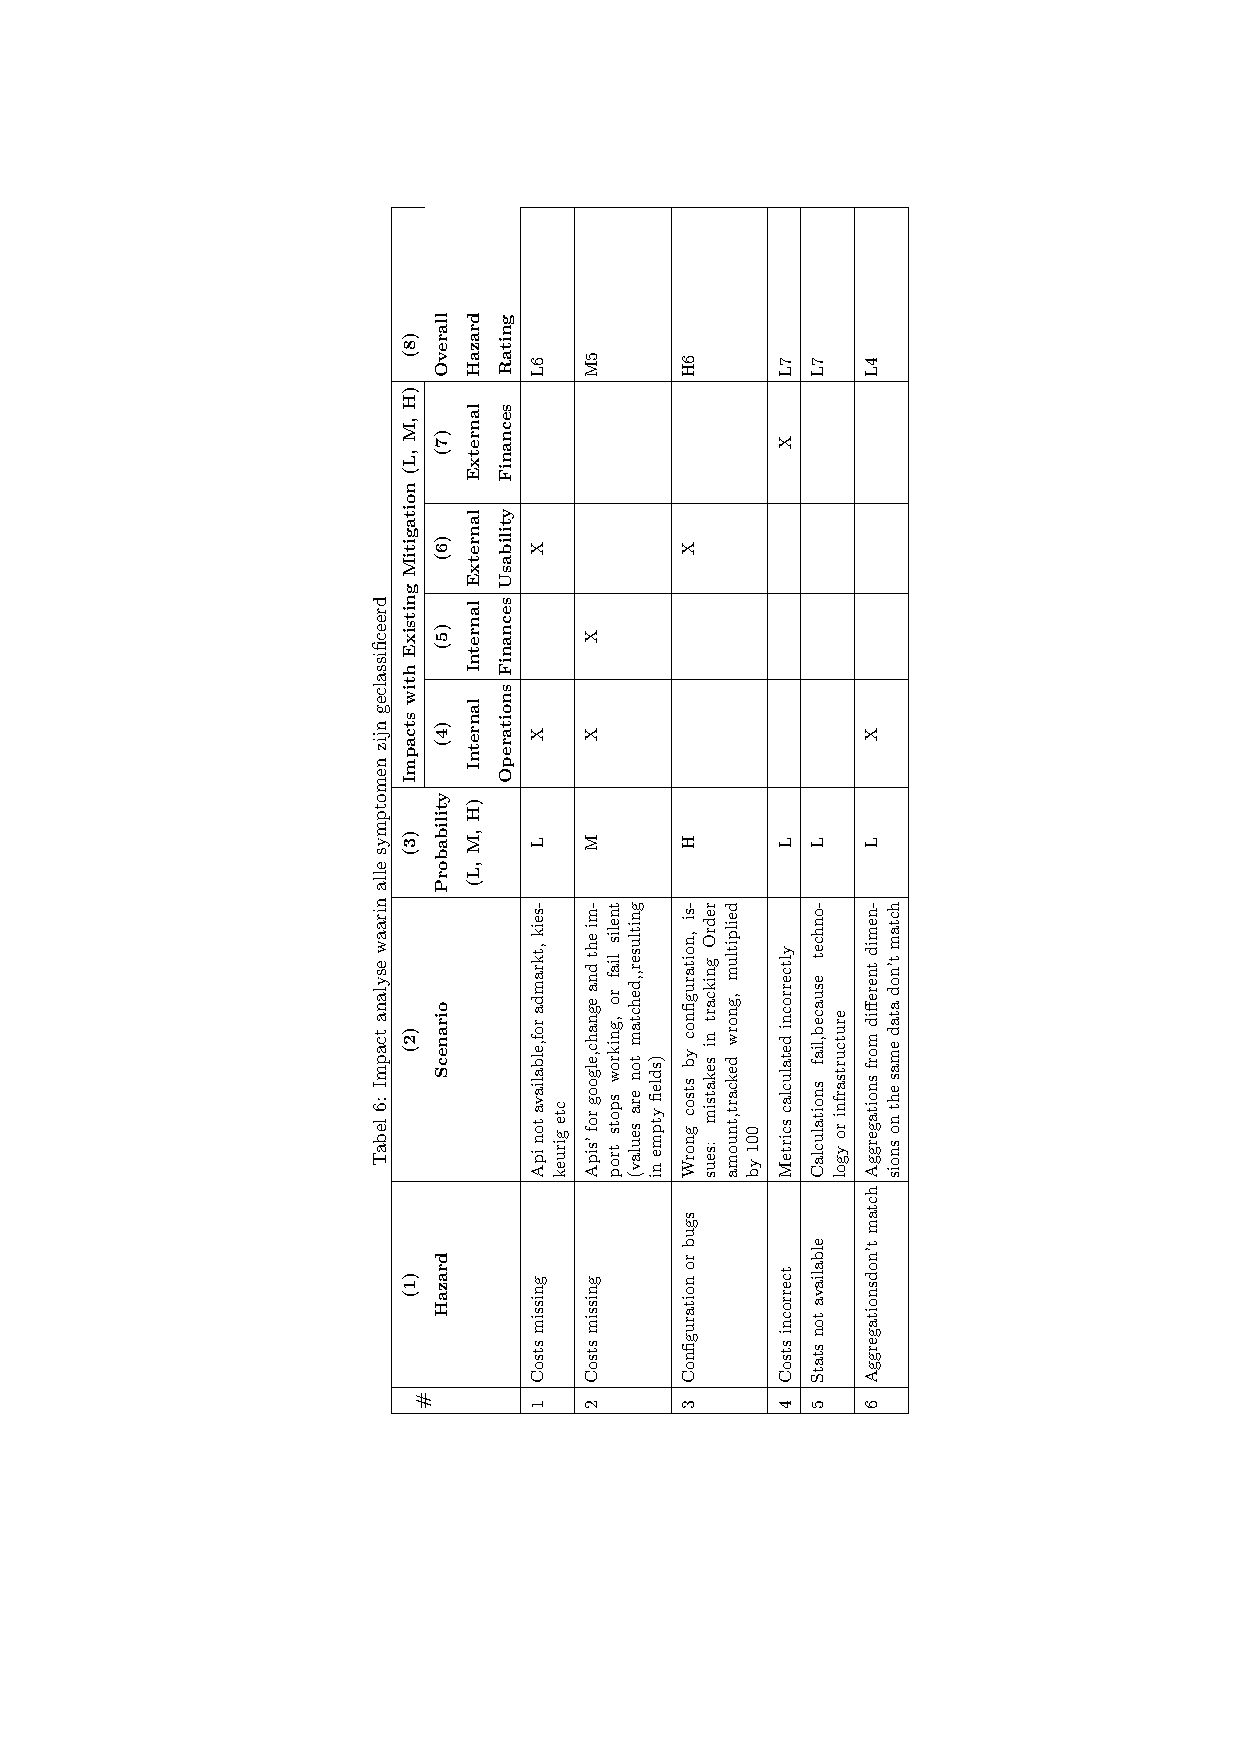
\includepdf[pages={1,2}]{appendix/impact-analyse-A.pdf}

\chapter{Implementatie ETL}
\label{app:json_format}
Het ETL proces heeft ongeveer het volgende algoritme

\begin{enumerate}
    \item Extract / download bestanden van Amazon S3
    \item Transform / bewerk de bestanden op locale hardeschijf met de splitter implementatie in Golang waardoor een BSON of CSV formaat wordt omgezet naar JSON met een uniform schema.
    \item Load / het resultaat wordt weg geschreven naar de locale hardeschijf. In het ontwerp is er voor gekozen om data te partitioneren per \verb+shop_id+ voor later gebruik.
\end{enumerate}



Het ETL proces neemt de volgende input data zoals in figuur \ref{fig:visits.json_before_etl2}, en transformeert dit in een JSON formaat zoals in figuur \ref{fig:visits.json_after_etl}

\begin{figure}[bh]
\centering
\caption{Een voorbeeld van de input data gebruikt tijdens ETL}
\label{fig:visits.json_before_etl2}
\begin{tabular}{|l|l|l|l|l|l|}
\hline
timestamp  & time\_id & publisher\_id & shop\_id & shop\_product\_id & shop\_category\_id \\ \hline
1464154281 & 20160424 & 410         & 224      & 103774145         & 338790             \\ \hline
1464154306 & 20160424 & 61          & 910      & 108837485         & 6782117            \\ \hline
1464154314 & 20160424 & 410         & 224      & 100670758         & 9152995            \\ \hline
\end{tabular}
\end{figure}


\begin{figure}[htb]
% \centering
\caption{De bestanden en hun formaat na het ETL proces door de Splitter}
\label{fig:visits.json_after_etl}
\begin{verbatim}
/Users/stefano/dev/go-aggregate/exports/224/visits.json
{"TimeId":"20160424","OrderID":"","ShopID":224,"ChannelID":410,
"ShopProductID":103774145,"ShopCategoryID":338790,"Traffic":1,
 "Order":0,"Amount":0,"ExAmount":0,"Cost":0}\n
{"TimeId":"20160424","OrderID":"","ShopID":224,"ChannelID":410,
 "ShopProductID":100670758,"ShopCategoryID":9152995,"Traffic":1,
 "Order":0,"Amount":0,"ExAmount":0,"Cost":0}\%
    
/Users/stefano/dev/go-aggregate/exports/910/visits.json
{"TimeId":"20160424","OrderID":"","ShopID":910,"ChannelID":61,
 "ShopProductID":108837485,"ShopCategoryID":6782117,"Traffic":1,
 "Order":0,"Amount":0,"ExAmount":0,"Cost":0}\%
\end{verbatim}
\end{figure}

\chapter{Data partities}
\label{app:partities}
Hier wordt een uitdraai gegeven als bewijsvoering voor de data grootte nadat de ETL fase is uitgevoerd, omschreven in \ref{sec:etl}. Aan de linker kant is de data grootte weergegeven, daarnaast de data partities per ShopID.

\begin{verbatim}

 12K	exports/{1298,1334,1501,1519,1544,1554,1568,1576}
 16K	exports/{1018,1495,1542,881}
 20K	exports/{1040,1281,1302,1312,1524,1241}
 24K	exports/{1067,1204,1496,1583,1136,655}
 28K	exports/{1069,1071,1163,1185,1515,1521,996}
 32K	exports/{1299,1402,1520}
 36K	exports/{1096,1529,843}
 40K	exports/{1311,1532,1581,
 44K	exports/{1221,1335,1392}
 48K	exports/1279
 52K	exports/{1099,1193,1438,776}
 56K	exports/{1225,1556}
 60K	exports/{1186,1260,992}
 64K	exports/{1230,1305,1001}
 68K	exports/1272
 72K	exports/{1022,1175,1227,1290,1360,1557}
 76K	exports/{1097,1394,1561}
 80K	exports/{1019,1226,1271,1355,1395,762}
 88K	exports/967
 92K	exports/848
 96K	exports/1346
 100K	exports/{1166,1194}
104K	exports/870
112K	exports/{1400,1530,885}
116K	exports/1184
124K	exports/{465,842,987}
128K	exports/{488,995}
132K	exports/{1252,1517}
136K	exports/{1242,1297}
140K	exports/{1398,1569}
144K	exports/{1164,751}
156K	exports/{1268,1442}
160K	exports/1036
164K	exports/{1244,1488}
168K	exports/1269
176K	exports/{1158,1358,873}
188K	exports/{1289,464}
192K	exports/{1228,410}
1.0M	exports/{1259,524}
1.1M	exports/{1167,750,854}
1.3M	exports/968
1.4M	exports/{1357,1577}
1.7M	exports/{1336,845}
1.8M	exports/1086
2.0M	exports/{430,1201,263}
2.5M	exports/{1168,1270,224,825}
2.8M	exports/954
3.0M	exports/{104,328,841,483}
3.3M	exports/910
3.4M	exports/849
3.7M	exports/1234
4.0K	exports/{1020,1024,1125,1182,1231,1283,1285,1286,1288,1325,1419,1485,1491,1493,1498,1506,...}
4.4M	exports/727
4.5M	exports/{1214,49,856,117}
5.5M	exports/955
4.9M	exports/{555,498}
6.1M	exports/759
6.1M	exports/878
7.5M	exports/956
9.1M	exports/335
9.2M	exports/1219
10M	    exports/990
18M	    exports/1213
35M	    exports/884
73M	    exports/1106
\end{verbatim}

\chapter{Implementatie in Golang}
\label{app:golang_code}
\begin{comment}
het volgende algoritme is geïmplementeerd voor de data aggregatie:
Iedere regel die is uitgelezen uit een input bestand wordt gecommuniceerd in een goroutine.
Een ander goroutine leest leest dir 

een proces verwerkt het inlezen van data uit een bestand. Voor twee bestanden worden er twee concurrent processen gestart. 
Daarnaast is een een proces dat voor ieder bericht de functies uitvoert om iedere kolomn uit op te tellen aan het vorige resultaat.
het resultaat wordt opgeslagen in een mapping, waarbij iedere key één regel representeer in het eindresultaat. Iedere regel uit de data input met een overeenkomstige key, wordt opgezocht in de mapping, en alle alle waardes uit de kolommen worden opgeteld.

het volgende voorbeeld visualeerd de mapping:
\begin{verbatim}
{
 Key{TimeID: 19881231, ShopID: 117, ChannelID: 4}:  Result{Visits: 100, Orders: 6},
 Key{TimeID: 19881231, ShopID: 117, ChannelID: 110}: Result{Visits: 47, Orders: 6}
}
\end{verbatim}

De key bevat de volgende waarden:  en de waardes voor data zijn te omschrijven als

\end{comment}

Het algoritme heeft een aantal stappen en past het braodcast principe toe, waarbij meerdere consumers (voor iedere data bron een), communiceren naar een receiver (de aggregatie functie):


\begin{enumerate}
\item lees de inhoud van ieder bestand in een \textit{goroutine} (één proces per bestand)
\item decodeiedere regel met de json package, naar struct ExportRow{} 
\item communiceer iedere regel als een door middel van Go \textit{channels} (zie dataChannel in figuur \ref{fig:golang_code1})
\item met behulp van een andere \textit{goroutine} wordt er gewacht op een bericht en de data opgeteld in een \textit{struct} Record{} (zie figuur \ref{fig:golang_code2})
\end{enumerate}

\clearpage

\begin{figure}[h]
\caption{Golang code for reading the input data } \label{fig:golang_code1}
\begin{lstlisting}[language=Golang]
dec := json.NewDecoder(file)
go func() {
    message := &domain.ExportRow{}
    for {
        err := dec.Decode(&message)
        if err == io.EOF {
            file.Close()
            return
        } else if err != nil {
            panic(err)
        }
        dataChannel <- *message
    }
}()
\end{lstlisting}
\end{figure}

\begin{figure}[!h]
\caption{Golang code for aggregating and writing output data }
\label{fig:golang_code2}
\begin{lstlisting}
r := map[Key]*domain.Record{}
go func() {
	for {
		dat := <-dataChannel
		key := Key{TimeId: dat.TimeId, ShopID: dat.ShopID}
		if r[key] == nil {
			r[key] = &domain.Record{TimeId: dat.TimeId, ShopProductID: dat.ShopProductID}
		}
		var rec *domain.Record = r[key]
		rec.ExAmount += dat.ExAmount
		rec.Amount += dat.Amount
		rec.Orders += dat.Order
		rec.Traffic += dat.Traffic
	}
}()
\end{lstlisting}
\end{figure}


\chapter{Implementatie in Spark SQL}
\label{app:spark_code}

\begin{figure}[h]
\caption{Python code for reading input and aggregating }
\begin{lstlisting}[language=python]
SQLContext(sc).read.json(args.inputFile).registerTempTable("s2m_mapped")
query = """
SELECT ShopID, ChannelID, ShopProductID,
       sum(Traffic) as traffic, sum(`Order`) as orders, sum(Cost) as costs
FROM s2m_mapped
WHERE TimeId={timeId}, ChannelID={channelId}
GROUP BY ShopID, ChannelID, ShopProductID
""".format(timeId=args.timeId, channelId=args.channelId)
job = sqlContext.sql(query)
job.write.partitionBy('ShopID').json(pathPrefix)
\end{lstlisting}
\end{figure}


\printbibliography

\end{document}